\section{Matplotlib}

%Matplotlib is a plotting library. In this section give a brief introduction to the matplotlib.pyplot module, which provides a plotting system similar to that of MATLAB.

Matplotlib 是一个绘图库。这里简要介绍matplotlib.pyplot模块,功能和MATLAB的绘图功能类似。

\subsection{Plotting}

%The most important function in matplotlib is plot, which allows you to plot 2D data. Here is a simple example:

matplotlib中最重要的函数是 \lstinline|plot|,该函数允许你绘制 2D 图形。这是一个简单的例子:
\lstinputlisting[]{code/matplotlib_plot.py}

%Running this code produces the following plot:

运行该代码可生成下图:
\begin{figure}[htbp]
        \centering
        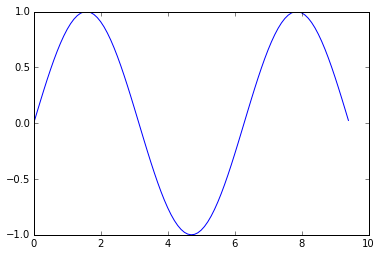
\includegraphics[width=3in]{images/sine.png}
\end{figure}



%With just a little bit of extra work we can easily plot multiple lines at once, and add a title, legend, and axis labels:

只需少量工作,就可以一次绘制多条曲线,并添加标题、图示和轴标:
\lstinputlisting[]{code/matplotlib_plot1.py}

\begin{figure}[htbp]
        \centering
        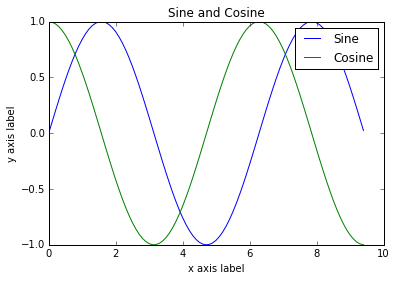
\includegraphics[width=3in]{images/sine_cosine.png}
\end{figure}


\subsection{Subplots}

%You can plot different things in the same figure using the subplot function. Here is an example:

可以使用 \lstinline|subplot| 函数来在一幅图中画不同的东西:  

\lstinputlisting[]{code/matplotlib_subplot.py}

\begin{figure}[htbp]
        \centering
        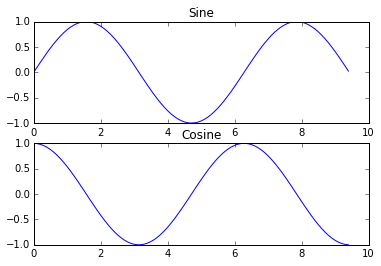
\includegraphics[width=3in]{images/sine_cosine_subplot.png}
\end{figure}


\subsection{Images}

%You can use the imshow function to show images. Here is an example:
你可以使用 \lstinline|imshow| 函数来显示图像。例如: 
\lstinputlisting[]{code/matplotlib_imshow.py}

\begin{figure}[htbp]
        \centering
        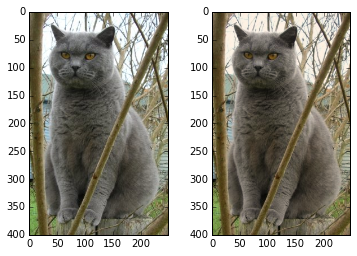
\includegraphics[width=4in]{images/cat_tinted_imshow.png}
\end{figure}
